\chapter{Konzeption}
\label{sec:chapter2}

Um die Zielsetzung zu erreichen, sind verschiedene Funktionalitäten erforderlich. Diese werden als Anforderungen definiert und in drei Kategorien unterteilt: 
\textbf{MUSS}, \textbf{SOLL} und \textbf{KANN}. Dadurch wird eine klare Priorisierung der Anforderungen ermöglicht. Zur Planung kommen Jira und verschiedene 
Diagrammtypen der \ac{UML} zum Einsatz. Die Anforderungen werden in Jira als Stories erfasst und einer Kategorie zugeordnet. Im Laufe der Entwicklung werden die Stories den 
jeweiligen Sprints zugewiesen. Diese Zuweisung erfolgt im wöchentlichen Rhythmus, um flexibel auf unerwartete Herausforderungen oder Hindernisse reagieren zu können.

\begin{table}[htb]
    \centering
    \renewcommand{\arraystretch}{1.3}
    \begin{tabular}{|p{4cm}|p{4cm}|p{4cm}|}
        \hline
        \multicolumn{3}{|c|}{\textbf{Anforderung}} \\ \hline
        \textbf{MUSS} & \textbf{SOLL} & \textbf{KANN} \\ \hline
        Bild/Video hochladen & Instagram-Login & Berechtigungsverwaltung \\ \hline
        Hinzufügen von Hashtags & Planung der Veröffentlichung & Automatische Anpassung von Medien \\ \hline
        Hinzufügen von Text & Responsive Design & Erinnerung an ausstehende Beiträge \\ \hline
    \end{tabular}
    \caption{Kategoriesierung der Anforderungen}
    \label{tab:tab-1}
\end{table}

\hyperref[tab:tab-1]{Tabelle 1} zeigt wie die Anforderungen in Kategorien unterteilt werden. Es handelt sich hierbei um besonders relevante Anforderungen aus
allen drei Kategorien. Eine vollständige Liste der Anforderung kann in Jira eingesehen werden.\footnote{Vgl. \url{https://engineeringproject.atlassian.net/jira/software/projects/SCRUM/boards/1}}

\begin{figure}[htb]
    \centering
    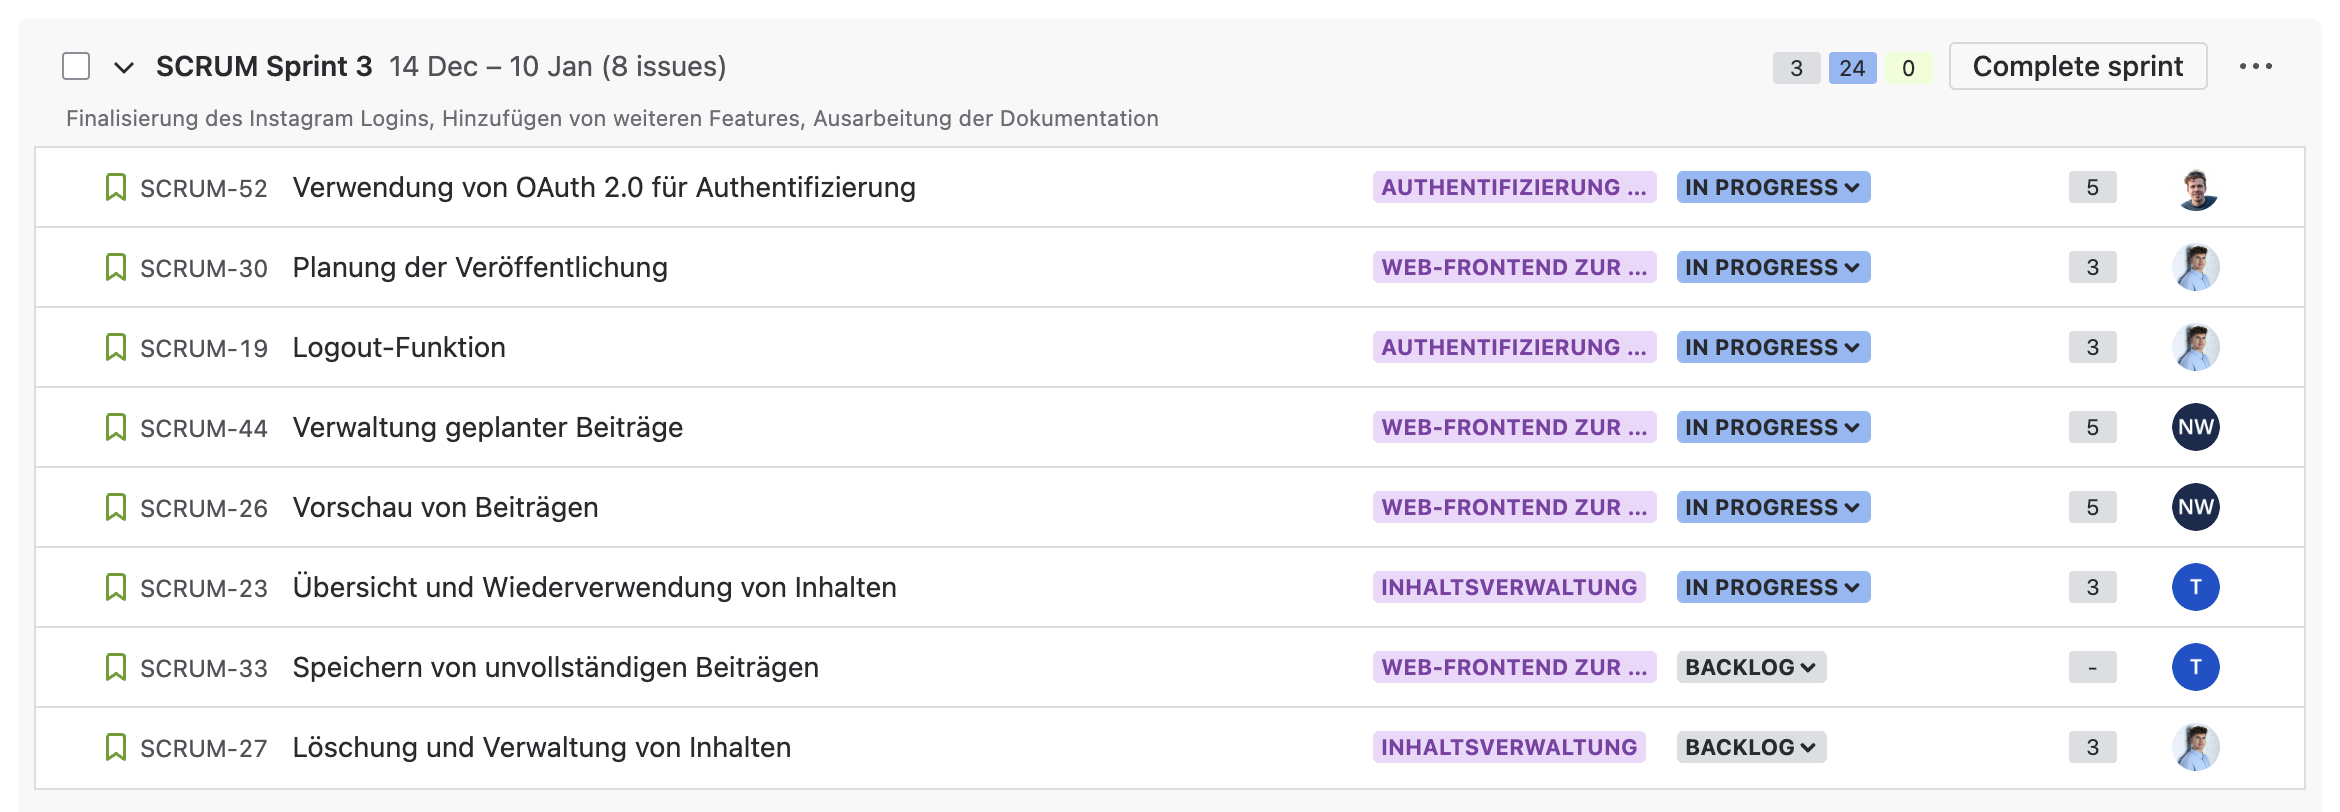
\includegraphics[width=0.8\textwidth]{graphics/sprint_3_jira.png}
    \caption{Sprint 3}
    \label{fig:fig-1}
\end{figure}

In \hyperref[fig:fig-1]{Abbildung 1} ist eine Übersicht von Sprint 3 zu sehen. Die Anzahl der Stories pro Sprint variiert je nach Komplexität und Umfang.
Die Entscheidung wie viele Stories in einen Sprint aufgenommen werden, wird im Team getroffen. Dabei wird darauf geachtet, dass die Stories in einem Sprint
realistisch umsetzbar und die Storypoints von Sprint zu Sprint annähernd gleich sind. Wird eine Storie in einem Sprint nicht fertiggestellt, wird sie in
den nächsten Sprint übernommen.

Die Definition der Anforderungen und die Planung der Sprints in Jira sind wesentliche Bestandteile des Projekts. Sie gewährleisten einen klaren Überblick über die 
Anforderungen und den Fortschritt während des gesamten Entwicklungsprozesses. Im Folgenden wird die technische Konzeption dargelegt.

\section{Technische Konzeption}
\label{sec:chapter2-1}

Im Rahmen der Entwicklung der Webanwendung wurden verschiedene Frameworks und Tools eingesetzt, um eine effiziente, flexible und 
skalierbare Lösung zu gewährleisten. Diese werden nachfolgend erläutert.

\textbf{Next.js}\footnote{Vgl. \cite{nextjs_docs}} wurde als zentrales Framework für die Entwicklung der Webanwendung verwendet. Es bietet leistungsstarke Funktionen wie Server-Side Rendering (SSR) 
und eine hohe Performance, wodurch die Ladezeiten optimiert werden. Zudem ermöglicht die Flexibilität von Next.js eine reibungslose Integration weiterer Technologien.

Für die Automatisierung der Instagram-Beiträge wird die offizielle \ac{API} von \textbf{Meta}\footnote{Vgl. \cite{facebook_graph_api}} genutzt. Diese erlaubt den Zugriff auf Beitragsdaten sowie die Planung von 
Posts, was die zentrale Funktion der Anwendung unterstützt.

Zur Implementierung einer modernen und modularen Benutzeroberfläche wurde \textbf{shadcn/ui}\footnote{Vgl. \cite{shadcn_ui_docs}} eingesetzt. Dieses UI-Framework zeichnet sich durch modulare Komponenten 
aus, die einfach erweiterbar sind. Zudem profitiert das Projekt von einer aktiven Community-Driven-Entwicklung, die regelmäßige Updates und Verbesserungen ermöglicht.

Für das Styling der Anwendung wurde \textbf{Tailwind CSS}\footnote{Vgl. \cite{tailwindcss_v2_docs}} verwendet. Der Utility-First-Ansatz erlaubt eine schnelle und konsistente Gestaltung der Benutzeroberfläche. Dank 
Responsive Design passt sich die Anwendung an verschiedene Bildschirmgrößen an. Zudem steigert Tailwind die Produktivität, da wiederverwendbare Klassen eine 
effiziente Entwicklung ermöglichen.

Zur sicheren und skalierbaren Verwaltung von Medieninhalten wurde \textbf{uploadthing} integriert. Dieses Tool bietet eine hohe Sicherheit für den Datei-Upload, eine 
nahtlose Next.js-Integration und eine gute Skalierbarkeit, um den wachsenden Anforderungen der Anwendung gerecht zu werden.

Diese beschriebenen Technologien bilden das Fundament der Webanwendung. Im nächsten Abschnitt wird die verwendete Architektur näher betrachtet.

\section{Architektur}
\label{sec:chapter2-2}

Um eine durchdachte und strukturierte Architektur zu gewährleisten, wurden zunächst verschiedene \ac{UML}-Diagramme erstellt. Diese dienen als 
Grundlage für die Implementierung und ermöglichen eine klare Strukturierung, aus der die einzelnen Komponenten der Anwendung abgeleitet werden können. Durch die 
Zusammenführung dieser Komponenten entsteht die Gesamtarchitektur der Anwendung.

\begin{figure}[htb]
    \centering
    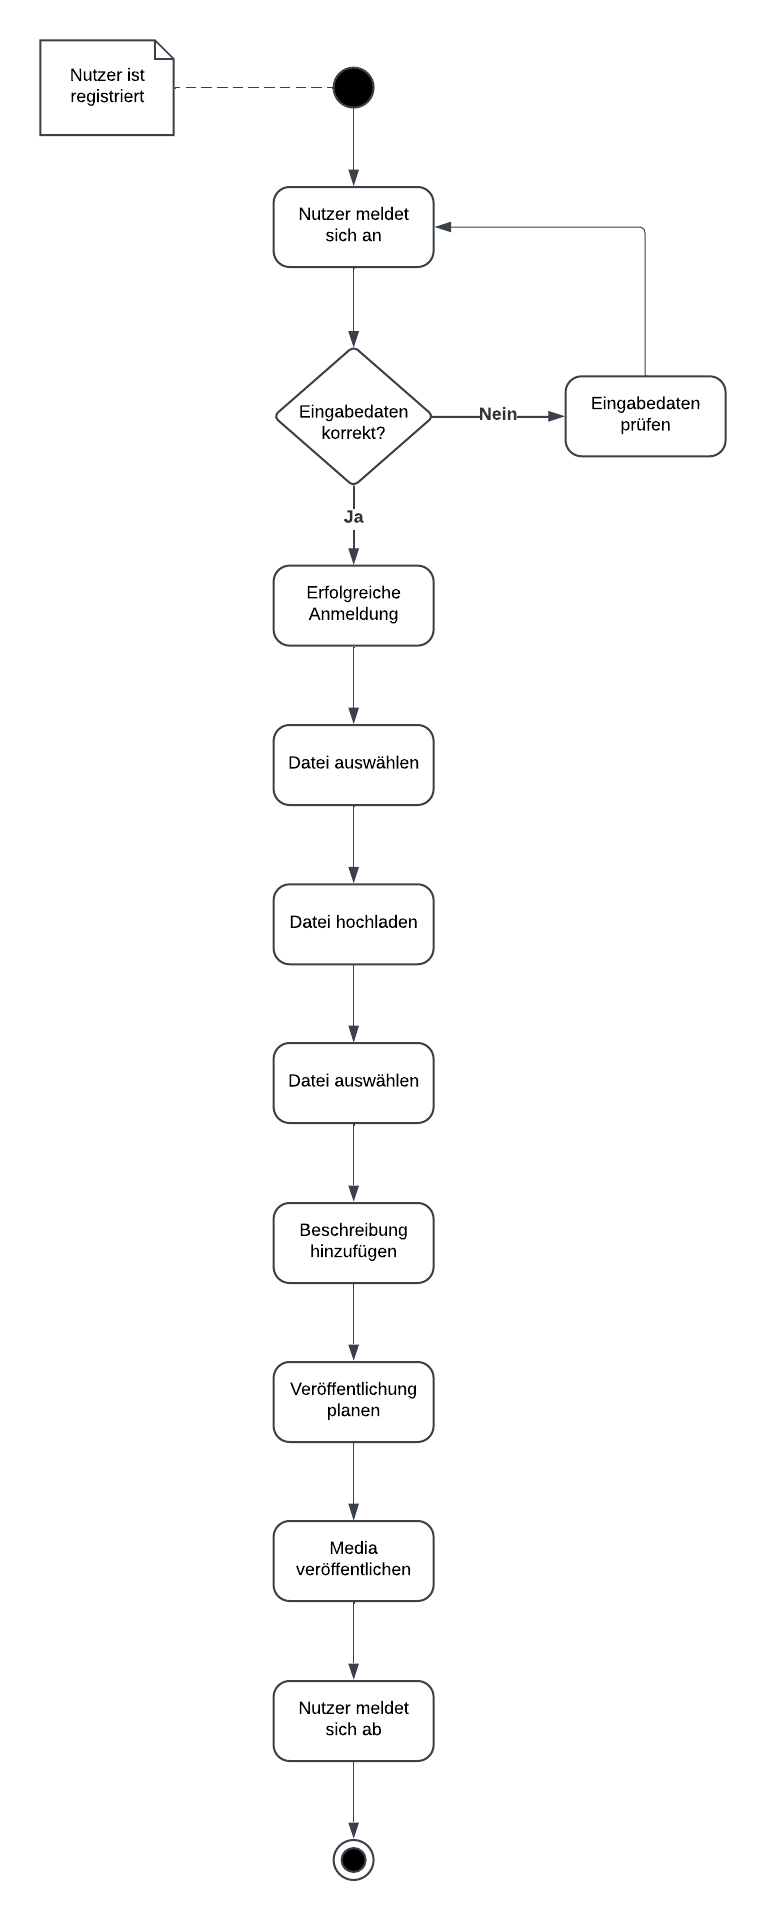
\includegraphics[width=0.8\textwidth, height=0.7\textheight]{graphics/activity_diagram.png}
    \caption{Aktivitätsdiagramm}
    \label{fig:fig-2}
\end{figure}
\clearpage

In \hyperref[fig:fig-2]{Abbildung 2} ist das \textbf{Aktivitätsdiagramm} dargestellt, das den typischen Ablauf der Benutzerinteraktion mit der Webanwendung zur 
automatisierten Veröffentlichung von Instagram-Beiträgen veranschaulicht. Es zeigt die einzelnen Schritte von der Anmeldung bis zur Veröffentlichung eines Beitrags 
und der anschließenden Abmeldung des Nutzers. Der Prozess beginnt mit einem bereits registrierten Nutzer, der sich in die Anwendung einloggt. Anschließend erfolgt 
eine Überprüfung der Eingabedaten. Falls diese nicht korrekt sind, wird der Nutzer zur erneuten Eingabe aufgefordert. Andernfalls erfolgt die erfolgreiche Anmeldung, 
und der Nutzer gelangt zur Hauptfunktionalität der Anwendung. Nach der Anmeldung kann der Nutzer eine Datei auswählen und diese anschließend hochladen. Dieser Schritt 
kann sich wiederholen, falls der Nutzer mehrere Dateien hochladen möchte. Anschließend wird eine Beschreibung hinzugefügt, um den Beitrag zu vervollständigen. Danach 
erfolgt die Planung der Veröffentlichung, bei der der Nutzer den gewünschten Veröffentlichungszeitpunkt festlegt. Sobald die Planung abgeschlossen ist, wird die 
Medienveröffentlichung durchgeführt. Abschließend meldet sich der Nutzer von der Anwendung ab, womit der Ablauf endet. Das Diagramm bietet eine strukturierte 
Darstellung der Benutzerinteraktion und stellt alle relevanten Schritte für eine erfolgreiche Beitragserstellung dar.

\begin{figure}[htb]
    \centering
    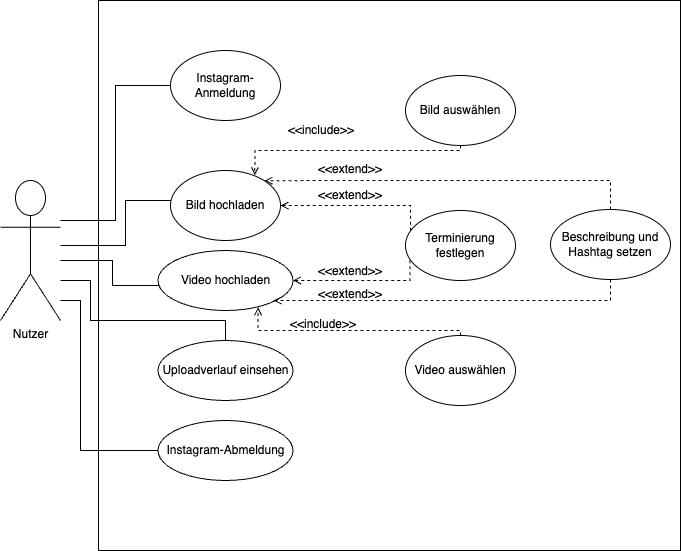
\includegraphics[width=0.8\textwidth]{graphics/use_case_diagram.png}
    \caption{Use Case Diagramm}
    \label{fig:fig-3}
\end{figure}

\hyperref[fig:fig-3]{Abbildung 3} stellt das \textbf{Use Case Diagramm} dar, das die wesentlichen Use Cases der Webanwendung beschreibt. Es zeigt die Interaktionen 
des Nutzers mit dem System und verdeutlicht die Beziehungen zwischen den einzelnen Anwendungsfällen. Der Nutzer kann sich zunächst über die Instagram-Anmeldung in 
die Anwendung einloggen.

Nach erfolgreicher Anmeldung stehen ihm mehrere Hauptfunktionen zur Verfügung:
\begin{itemize}
    \item Bild hochladen
    \item Video hochladen
    \item Uploadverlauf einsehen
    \item Instagram-Abmeldung
\end{itemize}

Die beiden Anwendungsfälle Bild hochladen und Video hochladen beinhalten jeweils optionale Erweiterungen (\textit{<<extend>>}):
\begin{itemize}
    \item Terminierung festlegen: Der Nutzer kann den Zeitpunkt der Veröffentlichung bestimmen.
    \item Beschreibung und Hashtags setzen: Zusätzlich kann er eine Bildbeschreibung und relevante Hashtags hinzufügen.
\end{itemize}

Zudem gibt es \textit{<<include>>}-Beziehungen, die darauf hinweisen, dass bestimmte Aktionen zwingend erforderlich sind:
\begin{itemize}
    \item Bild hochladen und Video hochladen beinhalten jeweils das Auswählen einer Datei (Bild oder Video), bevor der Upload erfolgen kann.
    \item Uploadverlauf einsehen ist ein separater Use Case, der dem Nutzer ermöglicht, eine Übersicht über bereits hochgeladene Inhalte zu erhalten.
\end{itemize}

Das Diagramm visualisiert die Modularität und Erweiterbarkeit der Anwendung, indem es optionale (\textit{<<extend>>}) und zwingend notwendige (\textit{<<include>>}) 
Abhängigkeiten zwischen den Use Cases darstellt. Dadurch wird eine strukturierte und skalierbare Architektur unterstützt.

\begin{figure}[htb]
    \centering
    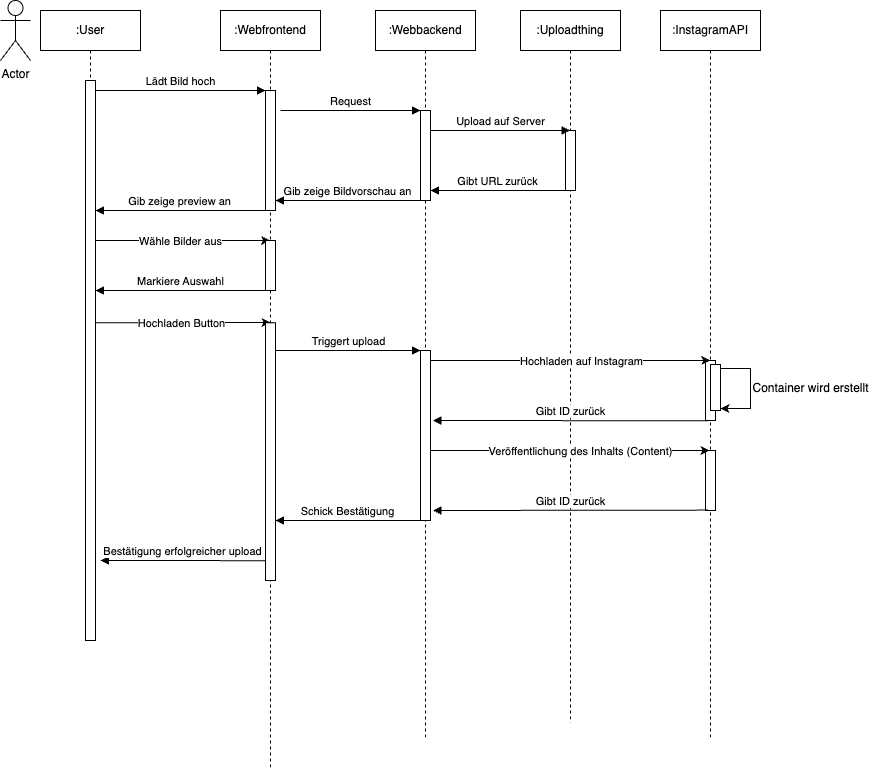
\includegraphics[width=0.8\textwidth]{graphics/sequence_diagram.png}
    \caption{Sequenzdiagramm}
    \label{fig:fig-4}
\end{figure}

In \hyperref[fig:fig-4]{Abbildung 4} ist das Sequenzdiagramm dargestellt, das den Ablauf für das Hochladen und Veröffentlichen eines Bildes in der Webanwendung beschreibt. Es zeigt die 
Interaktionen zwischen dem User, dem Webfrontend, dem Webbackend, dem Uploadthing-Service und der Instagram-\ac{API}. Im Folgeden wird der Ablauf der Interaktion beschrieben:

\begin{enumerate}
    \item \textbf{Nutzerinteraktion im Frontend}
    \begin{itemize}
        \item Der Nutzer lädt ein Bild hoch, indem er eine Vorschau anfordert.
        \item Das Webfrontend zeigt dem Nutzer eine Bildvorschau an, aus der er ein Bild auswählen und markieren kann.
        \item Nach Auswahl klickt der Nutzer auf den Hochladen-Button, um den Upload-Vorgang zu starten.
    \end{itemize}

    \item \textbf{Kommunikation zwischen Frontend und Backend}
    \begin{itemize}
        \item Das Webfrontend sendet eine Request-Nachricht an das Webbackend, um den Upload-Vorgang auszulösen.
    \end{itemize}

    \item \textbf{Upload auf Uploadthing}
    \begin{itemize}
        \item Das Webbackend kommuniziert mit dem Uploadthing-Service, um die Datei auf den Server hochzuladen.
        \item Nach erfolgreichem Upload gibt Uploadthing eine URL zurück, die die hochgeladene Datei referenziert.
    \end{itemize}

    \item \textbf{Verarbeitung durch die Instagram-\ac{API}}
    \begin{itemize}
        \item Das Webbackend verwendet die Instagram-\ac{API}, um das Bild zu veröffentlichen:
        \begin{itemize}
            \item Zuerst wird ein Container erstellt, um die Metadaten des Inhalts zu speichern.
            \item Anschließend wird das Bild hochgeladen, und die ID des Containers wird zurückgegeben.
            \item Die Veröffentlichung des Inhalts erfolgt, und die Content-ID wird zurückgegeben.
        \end{itemize}
    \end{itemize}

    \item \textbf{Bestätigung des erfolgreichen Uploads}
    \begin{itemize}
        \item Nach Abschluss aller Schritte sendet das Webbackend eine Bestätigung an das Webfrontend, welches dem Nutzer den erfolgreichen Abschluss des Uploads anzeigt.
    \end{itemize}
\end{enumerate}

Das Diagramm verdeutlicht den gesamten Workflow des Upload-Prozesses, einschließlich der Interaktionen zwischen verschiedenen Systemkomponenten. Es zeigt die Synchronität der Kommunikation 
und die Abhängigkeiten zwischen Frontend, Backend, externen Services und \acp{API}. Dies unterstützt die Entwickler bei der Implementierung und Fehlerbehebung des Upload- und Veröffentlichungsprozesses.


\begin{figure}[htb]
    \centering
    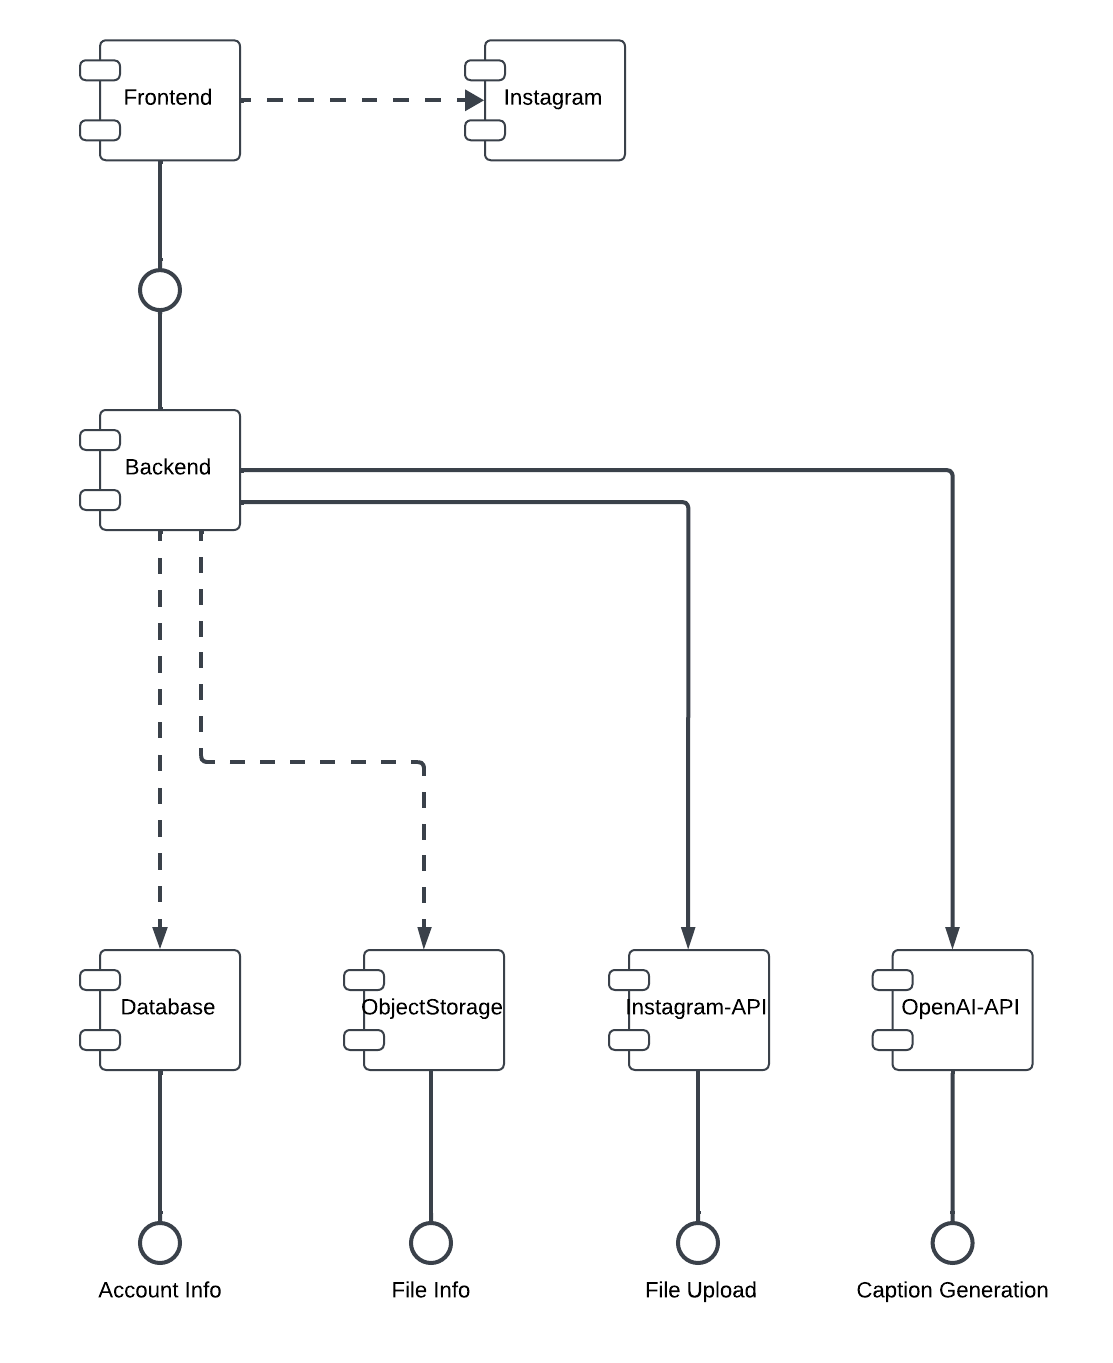
\includegraphics[width=0.8\textwidth]{graphics/components_diagram.png}
    \caption{Komponentendiagramm}
    \label{fig:fig-5}
\end{figure}

\hyperref[fig:fig-5]{Abbildung 5} zeigt das \textbf{Komponentendiagramm}, das die Architektur der Webanwendung beschreibt. Es zeigt die Hauptkomponenten sowie ihre Beziehungen und 
Abhängigkeiten zueinander. Nachfolgend werden die einzelnen Komponenten und ihre jeweiligen Funktionen beschrieben sowie die Beziehungen zwischen ihnen erläutert:
\clearpage

\begin{enumerate}
    \item \textbf{Frontend}
    \begin{itemize}
        \item Das Frontend stellt die Benutzeroberfläche bereit und ermöglicht die Interaktion des Nutzers mit der Anwendung.
        \item Es kommuniziert direkt mit der Instagram-Plattform, um Benutzeranmeldungen oder Beitragsvorschauen zu ermöglichen.
    \end{itemize}
    
    \item \textbf{Backend}
    \begin{itemize}
        \item Das Backend ist das zentrale Steuerungselement der Anwendung. Es verarbeitet die Daten aus dem Frontend und kommuniziert mit mehreren anderen Komponenten, darunter:
        \begin{itemize}
            \item Datenbank: Zum Speichern von Benutzerdaten, Beitragsinformationen und Metadaten.
            \item Object Storage: Für die sichere Speicherung hochgeladener Mediendateien wie Bilder oder Videos.
            \item Instagram-\ac{API}: Zum Veröffentlichen von Beiträgen oder Planen von Inhalten direkt auf Instagram.
            \item OpenAI-\ac{API}: Zur Generierung von Hashtags oder Beschreibungen basierend auf den hochgeladenen Inhalten.
        \end{itemize}
    \end{itemize}
    
    \item \textbf{Datenbank}
    \begin{itemize}
        \item Die Datenbank speichert strukturierte Daten wie Benutzerinformationen, geplante Veröffentlichungen und Protokolle der Anwendung.
    \end{itemize}
    
    \item \textbf{Object Storage}
    \begin{itemize}
        \item Der Object Storage dient der Speicherung und Verwaltung von Mediendateien wie Bildern und Videos, die mit Beiträgen verknüpft sind.
    \end{itemize}
    
    \item \textbf{Instagram-\ac{API}}
    \begin{itemize}
        \item Die Instagram-\ac{API} wird verwendet, um Inhalte auf Instagram zu veröffentlichen oder Interaktionen mit der Plattform zu ermöglichen.
    \end{itemize}
    
    \item \textbf{OpenAI-\ac{API}}
    \begin{itemize}
        \item Die OpenAI-\ac{API} wird verwendet, um KI-basierte Funktionen wie die Generierung von Textinhalten oder Vorschlägen für Hashtags bereitzustellen.
    \end{itemize}
\end{enumerate}

\textbf{Beziehungen zwischen den Komponenten}
\begin{itemize}
    \item Das Frontend kommuniziert direkt mit dem Backend, das als zentrales Gateway für alle weiteren Abhängigkeiten fungiert.
    \item Das Backend verbindet sich mit der Datenbank und dem Object Storage, um Inhalte zu speichern und zu verwalten.
    \item Die Instagram-\ac{API} und die OpenAI-\ac{API} erweitern die Funktionalität, indem sie externe Dienste integrieren.
\end{itemize}

Das Diagramm verdeutlicht die Modularität und Erweiterbarkeit der Anwendung und stellt sicher, dass die Komponenten klar voneinander getrennt sind, was die Wartbarkeit und Skalierbarkeit der 
Architektur unterstützt.
